

 
\chapter*{--------- BONFIRE HIT ---------}

谢谢你带我来到这里，伴火同进者，终有一天会遇见命定之死，永别了。



%%%%%%%%%%%%%%%%%%%%%%%%%%%%%%%%%%%%%%%%%%%%%% 毕业考试题一 %%%%%%%%%%%%%%%%%%%%%%%%%%%%%%%%%%%%%%%%%%%%%%%%%%%%%%%%%%%%%%%%%%%%%%%%%%%%
设计一个表示扑克牌的数据结构（无大小王），要求支持操作：给出\uline{至多}五张牌，判断其中最大的牌型是什么。\\

牌型大小排序如下：

同花顺 > 四条 > 葫芦 > 同花 > 顺子 > 三条 > 两对 > 一对 > 高牌。

同花顺：同时满足“同花”和“顺子”，见下。

四条：存在四张相同的牌，如6,6,6,6,3；8,8,8,8,K等；

葫芦：其中三张相同，另外两张相同，如8,8,8,2,2，A,A,A,Q,Q等；

同花：必须由五张花色相同的牌组成；

顺子：必须由五张点数紧挨着的牌组成，如A,2,3,4,5、10,J,Q,K,A、6,7,8,9,10等；

高牌：无其他牌型。如：非同花的A,9,J,10,6，4,5,6,7,9等。\\

如：\\
1）输入：
\begin{center}
    
\includegraphics[width=0.66\textwidth]{assets/pics_and_ppts/others/毕业考试01扑克牌输入示例一.png}
\end{center}
输出：高牌。\\
2）输入：
\begin{center}
    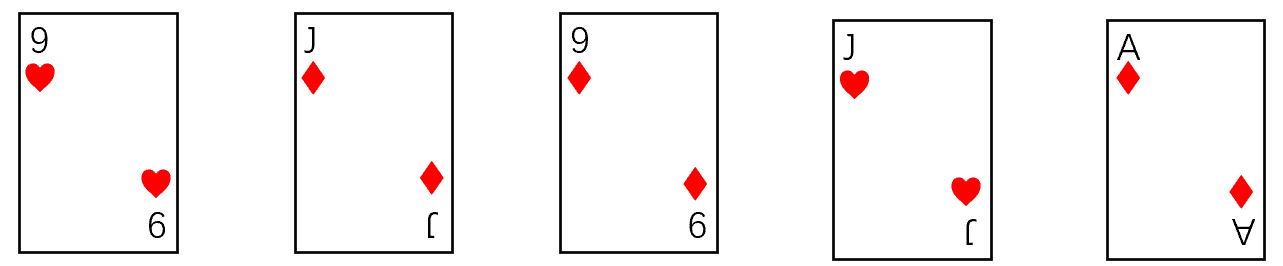
\includegraphics[width=0.63\textwidth]{assets/pics_and_ppts/others/毕业考试01扑克牌输入示例二.png}
\end{center}
输出：两对。\\
3）输入：
\begin{center}
    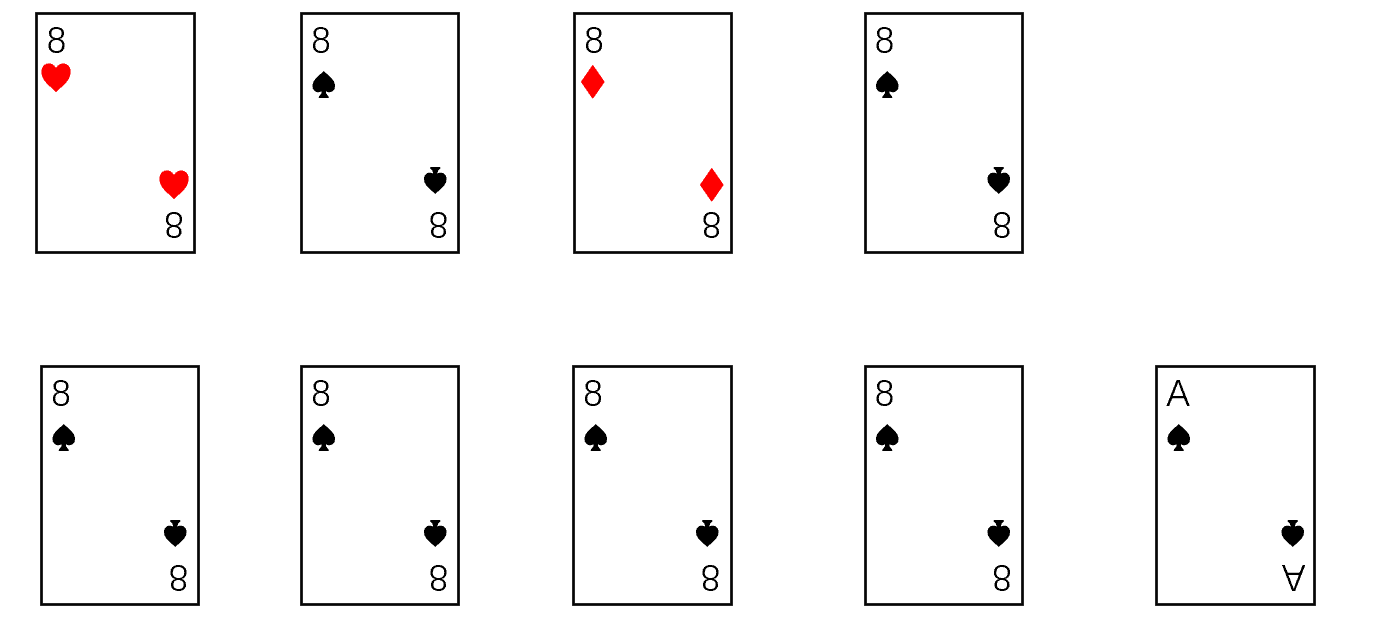
\includegraphics[width=0.63\textwidth]{assets/pics_and_ppts/others/毕业考试01扑克牌输入示例三.png}
\end{center}
输出：四条。



%%%%%%%%%%%%%%%%%%%%%%%%%%%%%%%%%%%%%%%%%%%%%% 毕业考试题二 %%%%%%%%%%%%%%%%%%%%%%%%%%%%%%%%%%%%%%%%%%%%%%%%%%%%%%%%%%%%%%%%%%%%%%%%%%%%





